\chapter{Result}
\label{Result}
\textit{This chapter presents the evaluation results. Appendix \ref{appendix:raw} contains complemented data and metrics which will not be shown in this chapter. The chapter starts with exposing the results of the \textit{\nameref{Applications}} evaluation. This follows by results presented from the \textit{\nameref{Performance}} evaluation.}



\section{Web Applications}
\label{Applications}
The results presented in this section are from evaluating Java applications for security vulnerabilities with and without WebTaint. The results from each application are listed in tables where vulnerability type and the vulnerability count are presented.

Table \ref{table:MicroTable} shows the vulnerabilities from evaluating Stanford SecuriBench Micro \parencite{securiBenchMicro}. In the table can we see that the most common vulnerability is Reflected Cross-Site Scripting where 71 vulnerabilities are presented. Second most common is SQL Injection with 20 and the least common with one vulnerability is Buffer Overflow. By enabling WebTaint on the Stanford SecuriBench Micro \parencite{securiBenchMicro} application results in a 100\% prevention rate.

\begin{table}[H]
  \centering
  \caption{Security vulnerabilities detected by WebTaint in Stanford SecuriBench Micro}
  \label{table:MicroTable}
    \begin{tabular}{rcc}
      & \textbf{Vulnerabilities} & \textbf{Detected by WebTaint} \\
      \textbf{\begin{tabular}[c]{@{}r@{}}Cross-Site Scripting\\ (Reflected)\end{tabular}} & 71            & 71  \\
      \textbf{SQL Injection}                    & 20            & 20  \\
      \textbf{Buffer Overflow}                  & 1             & 1  
    \end{tabular}
\end{table}

Table \ref{table:InsecureTable} shows the vulnerabilities from running the InsecureWebApp \parencite{insecure} with and without WebTaint. Of the two types of vulnerabilities is SQL Injection the most common with six vulnerabilities and Reflected Cross-Site Scripting with two. Enabling WebTaint on the InsecureWebApp \parencite{insecure} results in 100\% prevention rate on SQL Injection attacks and 0\% for Cross-Site Scripting. The overall prevention rate is 75\%. 

\begin{table}[H]
  \centering
  \caption{Security vulnerabilities detected by WebTaint in InsecureWebApp}
  \label{table:InsecureTable}
    \begin{tabular}{rcc}
      & \textbf{Vulnerabilities} & \textbf{Detected by WebTaint} \\
      \textbf{\begin{tabular}[c]{@{}r@{}}Cross-Site Scripting\\ (Reflected)\end{tabular}}      & 2             & 0  \\
      \textbf{\begin{tabular}[c]{@{}r@{}}SQL Injection -\\ Authentication Bypass\end{tabular}} & 2             & 2  \\
      \textbf{\begin{tabular}[c]{@{}r@{}}SQL Injection -\\ Hypersonic SQL\end{tabular}}       & 4             & 4  
    \end{tabular}
\end{table}

Table \ref{table:Ticketbook} shows the vulnerabilities from evaluating the Ticketbook \parencite{ticketbook}. The most common vulnerability was the Cross-Site Scripting with 14 occurrences. The SQL Injection was the least with one. The prevention rate of the SQL Injection was 100\% and for Cross-Site Scripting 71.4\% when enabling WebTaint. The overall prevention rate is 73.3\%.

\begin{table}[H]
  \centering
  \caption{Security vulnerabilities detected by WebTaint in Ticketbook}
  \label{table:Ticketbook}
  \begin{tabular}{ccc}
    & \textbf{Vulnerabilities} & \textbf{Detected by WebTaint} \\
    \textbf{\begin{tabular}[c]{@{}r@{}}Cross-Site Scripting\\ (Persistent)\end{tabular}} & 2             & 2 \\
    \textbf{\begin{tabular}[c]{@{}r@{}}Cross-Site Scripting\\ (Reflected)\end{tabular}}  & 12            & 8 \\
    \textbf{SQL Injection}                     & 1             & 1
  \end{tabular}
\end{table}

The results from evaluating the application SnipSnap \parencite{snipsnap} is seen in Table \ref{table:SnipSnapTable}. In this table can we see that the most common vulnerability is the Reflected Cross-Site Scripting with 172 occurrences. Second highest is the SQL Injection with 49 occurrences followed by the CRLF Injection with two. Enabling WebTaint yields an overall prevention rate of 77.2\%. All CRLF Injection is prevented. The Cross-Site Scripting prevented with 77.3\% and the SQL Injection with 75.5\%.

\begin{table}[H]
  \centering
  \caption{Security vulnerabilities detected by WebTaint in SnipSnap}
  \label{table:SnipSnapTable}
  \begin{tabular}{rcc}
    & \textbf{Vulnerabilities} & \textbf{Detected by WebTaint} \\
    \textbf{\begin{tabular}[c]{@{}r@{}}Cross-Site Scripting\\ (Reflected)\end{tabular}}      & 172           & 133  \\
    \textbf{CRLF Injection}                        & 3             & 3    \\
    \textbf{SQL Injection}                         & 47            & 37   \\
    \textbf{\begin{tabular}[c]{@{}r@{}}SQL Injection -\\ Authentication Bypass\end{tabular}} & 2             & 0       
  \end{tabular}
\end{table}

The results indicate that detection and prevention of the SQL Injection and the Criss-Site Scripting attacks are possible. Detection of vulnerabilities is possible for all applications and the average prevention rate for all four applications is 81\%.

\section{Introduced Overhead}
\label{Performance}
The results from benchmarking the application on the DaCapo Benchmark Suit \parencite{dacapo} is seen in Figure \ref{fig:Time} and \ref{fig:Memory}. Both graphs are constructed to show the added overhead of running the applications with WebTaint enabled. The graphs are constructed based on the data in Table \ref{TimeTable} and \ref{MemoryTable} in appendix \ref{appendix:raw}.



\subsection{Time}
Figure \ref{fig:Time} displays the results of the average time overhead per application when enabling WebTaint. The results show that the application with the least average time overhead was the Tradesoap where 14.7\% was added. The application with the most average time overhead was the Batik with an overhead of 432.2\%. The average overall is 162.9\%.

\begin{figure}[H]
    \centering
    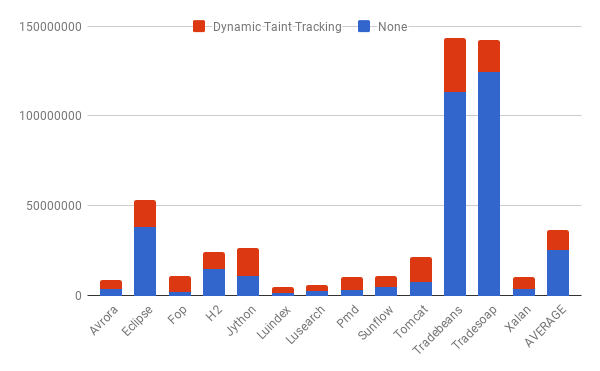
\includegraphics[width=\textwidth]{images/Time.png}
    \caption{Average added time in microseconds}
    \label{fig:Time}
\end{figure}



\subsection{Memory}
Figure \ref{fig:Memory} displays the results of the average memory overhead per application. The results show that the application with the least average memory overhead was the Eclipse where 5.5\% was added. The largest application was the Batik with an overhead of 344.6\%. The average overall is 142.7\%.

\begin{figure}[H]
    \centering
    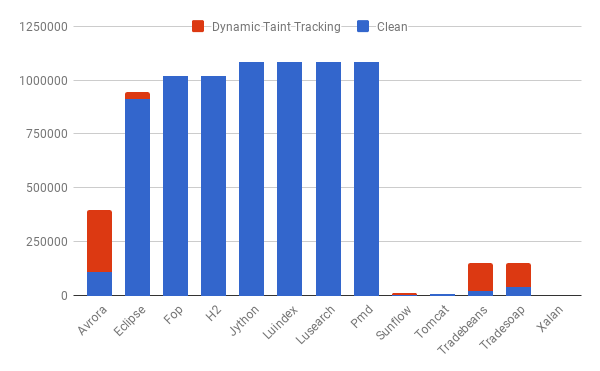
\includegraphics[width=\textwidth]{images/Memory.png}
    \caption{Average added memory in kilobytes}
    \label{fig:Memory}
\end{figure}